\chapter{Introduction into bacterial interactions}
Interactions in natural microbial communities are a very common phenomenon~\cite{Weiland-Brauer2021-eq, Braga2016-fr}, yet replicating such communities in a controlled environment is challenging, and therefore the impact of such interactions on single species or whole communities is often overlooked. The most simple interaction which is also implemented in controlled environments is resource competition which indirectly limits the growth of other members of the community. However, whenever we use the word interaction in this thesis, we mean more direct interactions. Many different kinds of interactions are known such as symbiotic interactions, where one microorganism produces some compound essential for another memeber of the community to grow.~\cite{Sarsan2021-pn} We focus in this work on antagonistic interactions. These are interactions where one interaction partner harms the other's growth to gain a benefit itself. We are studying in this thesis two of the most known antagonistic interactions in two different projects. In a first, experimental project, we are studying selection and evolution of antibiotic production and in the second, modeling project, we study the impact of resistant competitors on bacteria-phage interactions.~Figure~\ref{fig:intro_shared_interactions} sketches the two interactions and projects we are presenting here.

\begin{figure}
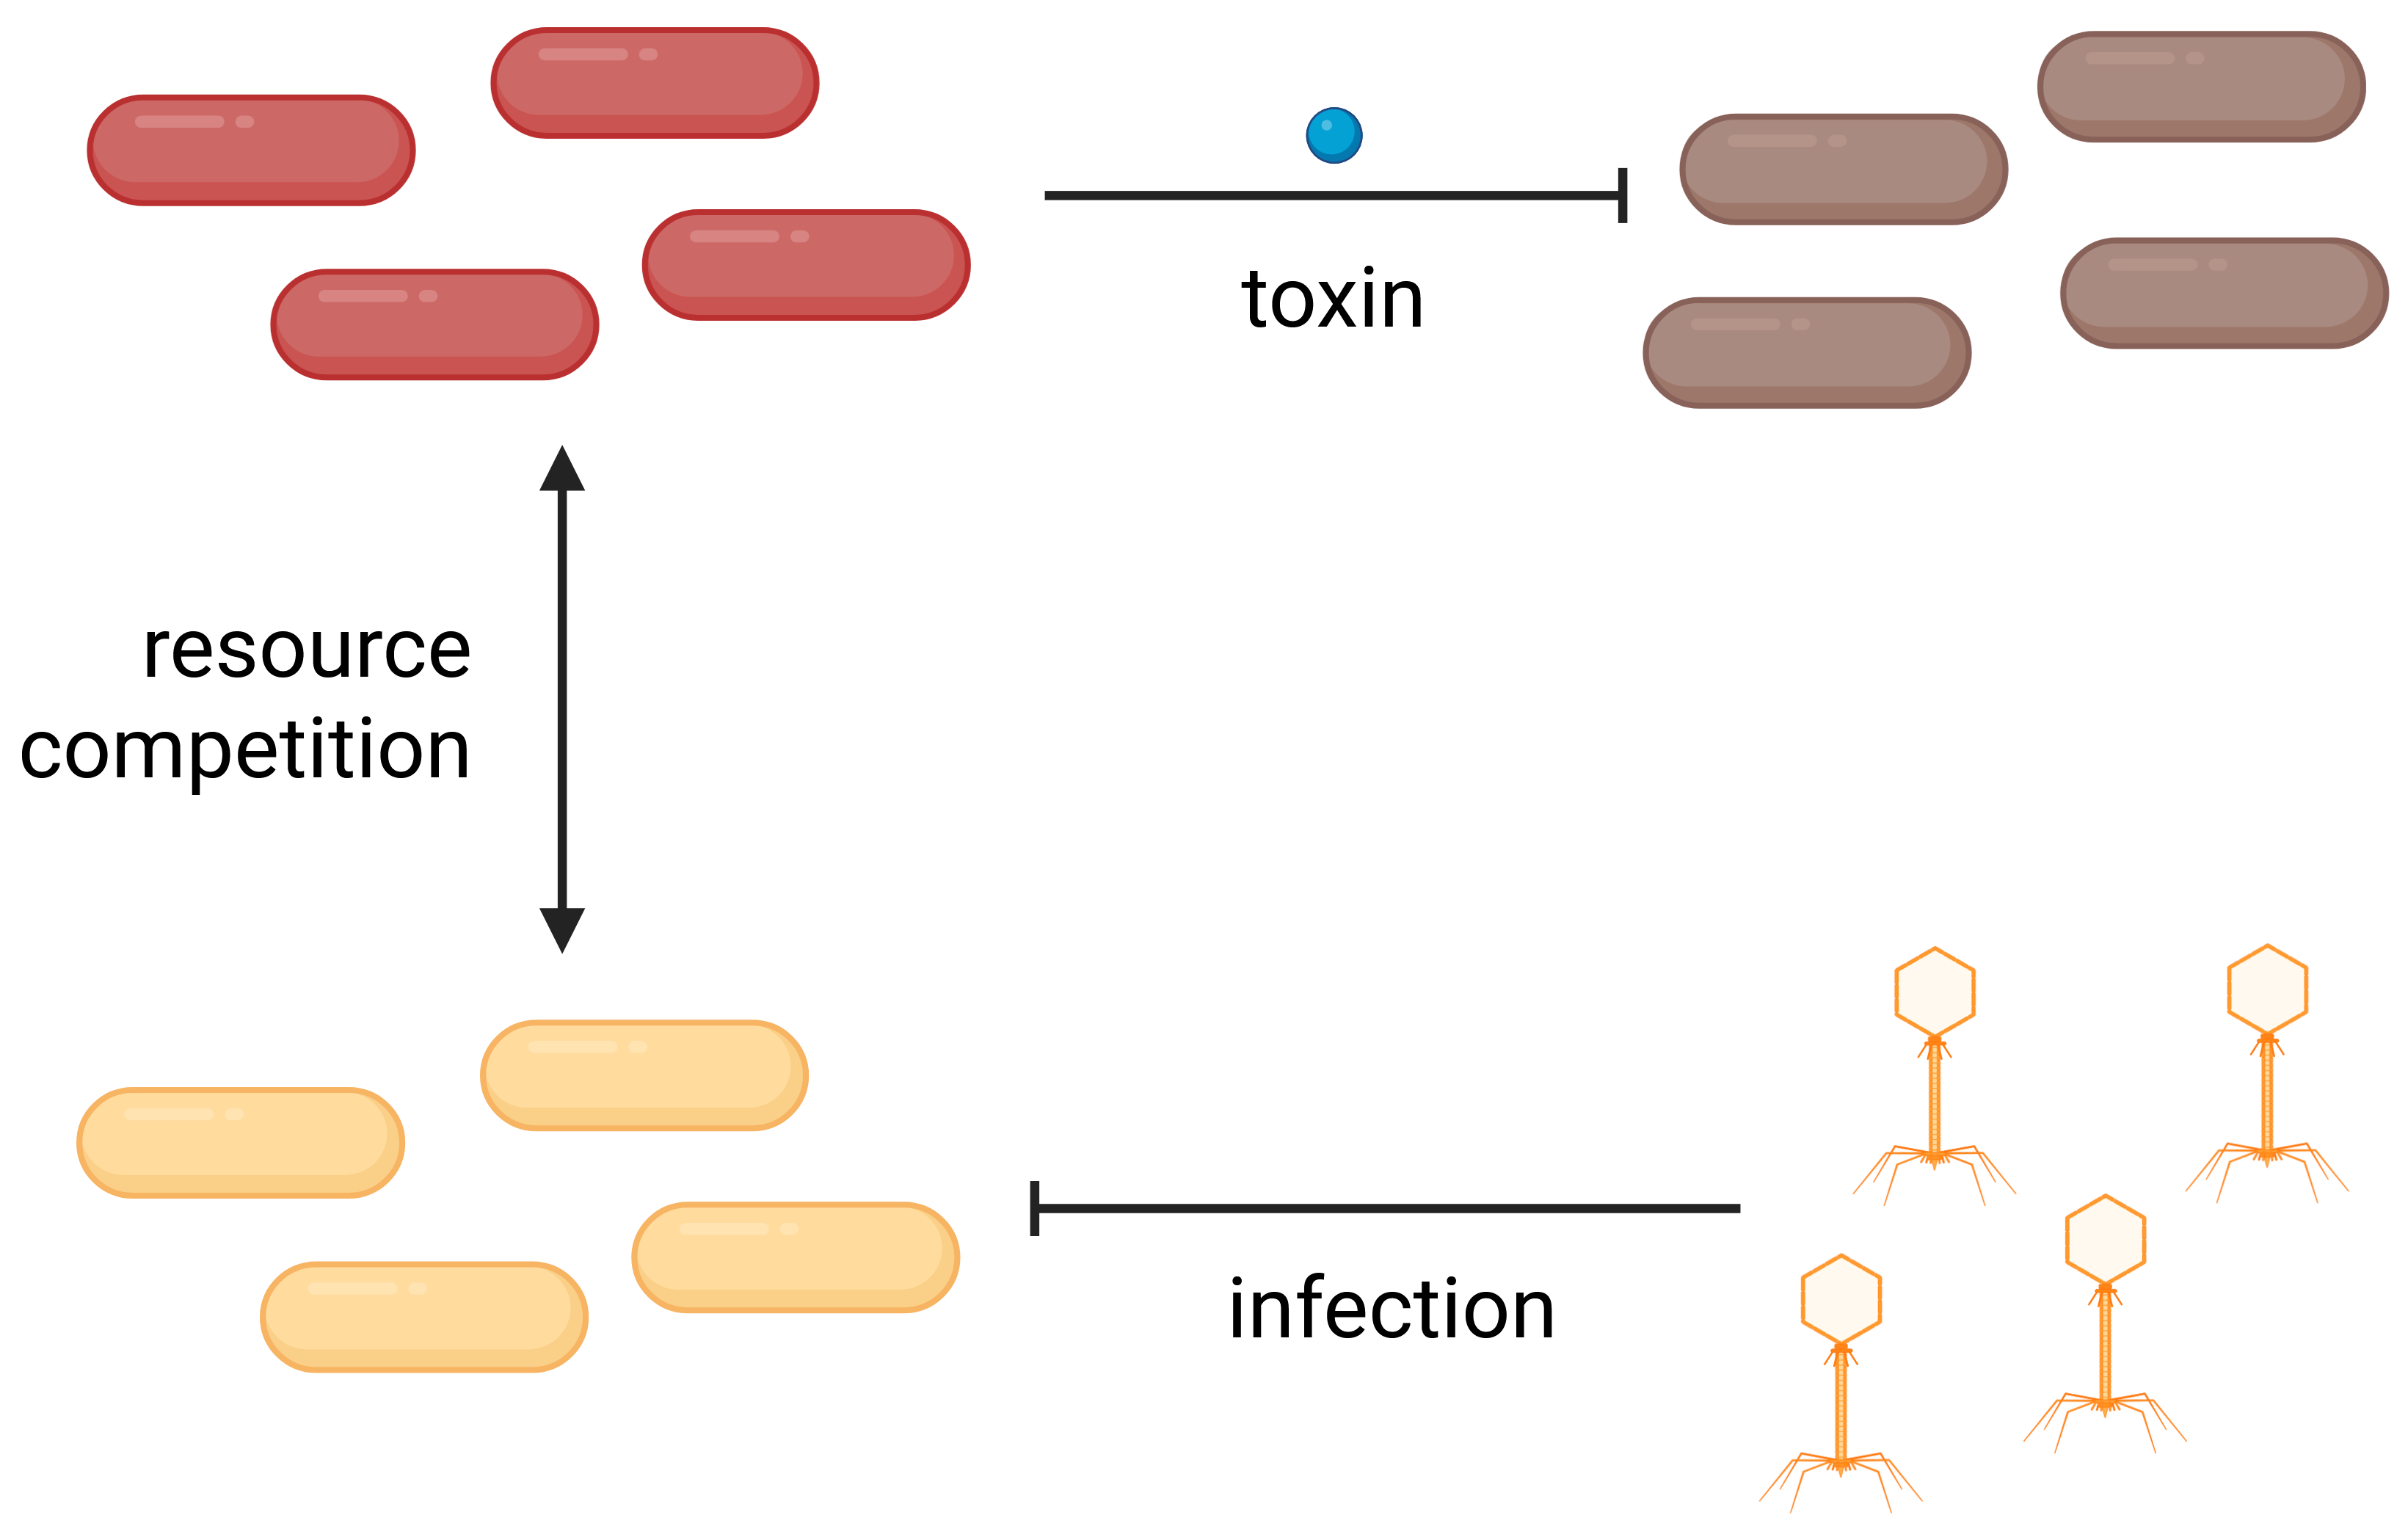
\includegraphics[width=\linewidth]{graphics/2025_09_30_intro_fig1.png}
\caption{\textbf{Antagonistic interactions studied in projects in this thesis} This sketch shows two common antagonistic interactions in microbial communities. The upper part of the sketch shows the production of a toxin by a bacterial population which can then inhibit another target strain, sensitive to the produced toxin. At the same time there are other members in the community which compete for available resources such as nutrients. This interaction will be studied in the first, experimental project of this thesis. The lower part of the sketch shows the infection of a bacterial species by phages. Phage infections form an integral, important part of natural ecology. In addition to the phage infection threat, the bacteria are in resource competition with phage-resistant bacteria. This bacteria-phage interaction will be studied in the second, theoretical project of this thesis.}
\label{fig:intro_shared_interactions}
\end{figure}